% !TEX root = ../thesis.tex

\chapter{Case Study II: Medical Ultrasound Diagnosis} \label{chp:medical}

\section{Clinical Problem Statement}

Medical ultrasound diagnosis represents an ideal validation domain for L2 Predictive Twin capabilities, offering complex reasoning challenges that require sophisticated model orchestration and uncertainty quantification. This domain demands integration of visual information, clinical data, and predictive modeling to support evidence-based diagnostic decisions.

The diagnostic complexity in medical imaging stems from the inherent ambiguity and variability in ultrasound images, which require expert interpretation to identify subtle patterns and abnormalities. Unlike automated image classification tasks, clinical diagnosis involves understanding pathophysiological processes, considering patient history and symptoms, and quantifying uncertainty in diagnostic conclusions. This complexity makes the domain particularly suitable for demonstrating the value of cognitive architectures over traditional AI approaches.

Current limitations in medical AI include narrow focus on single-modal analysis that ignores clinical context, lack of uncertainty quantification in diagnostic outputs, poor integration with existing clinical workflows, and limited ability to explain diagnostic reasoning in clinically meaningful terms. These limitations highlight the need for more sophisticated approaches that can integrate multiple information sources while providing reliable, interpretable diagnostic support.

The clinical environment presents unique challenges including strict safety and regulatory requirements, need for seamless integration with existing hospital systems, requirement for real-time responsiveness during clinical procedures, and necessity for clear, actionable diagnostic outputs that support clinical decision-making rather than replacing physician judgment.

\section{Predictive Twin Design and CORTEX Adaptation}

The non-visual Digital Twin architecture for medical ultrasound represents a novel approach that focuses on clinical reasoning rather than direct image analysis. This design choice addresses fundamental limitations in current medical AI approaches while enabling more robust and clinically relevant diagnostic support.

\begin{figure}[htbp]
\centering
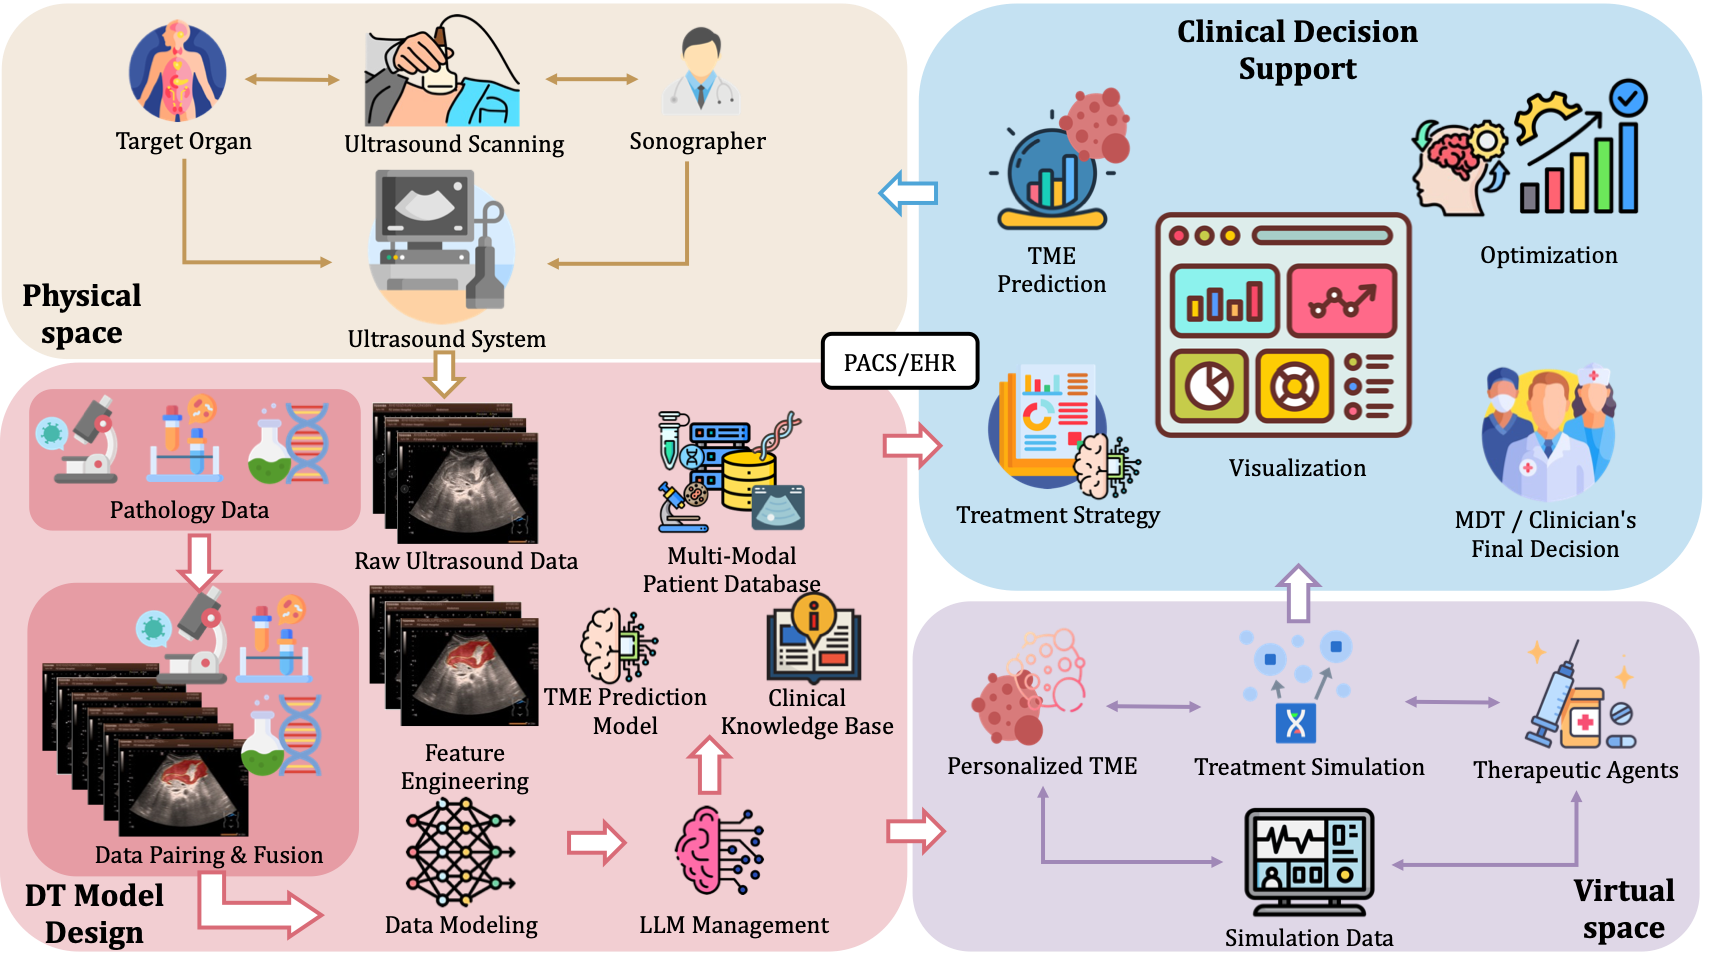
\includegraphics[width=0.8\textwidth]{Med/med_framework.png}
\caption{Digital Twin architecture framework for medical ultrasound diagnosis. The framework shows the complete workflow from ultrasound scanning in physical space to clinical decision support in virtual space, including data pairing and fusion, Digital Twin model design, feature engineering, TME prediction model, and LLM management components.}
\label{fig:med_framework}
\end{figure}

The architectural approach emphasizes structured feature extraction from ultrasound images using established computer vision techniques, integration of extracted features with clinical data and patient history, application of validated medical models for risk assessment and prediction, and synthesis of results into clinically actionable diagnostic insights. This approach leverages the strengths of both computer vision and clinical reasoning while avoiding the limitations of end-to-end black-box approaches.

Feature extraction employs established medical imaging techniques including segmentation algorithms validated for ultrasound analysis, quantitative measurements of anatomical structures and abnormalities, texture analysis to characterize tissue properties, and morphological assessment to identify structural anomalies. These features provide objective, quantifiable inputs for subsequent reasoning processes while maintaining clinical interpretability.

Clinical integration involves combining extracted image features with patient demographics, medical history, current symptoms, laboratory results, and relevant clinical guidelines. This integration ensures that diagnostic reasoning considers the full clinical context rather than relying solely on imaging data. The approach mirrors established clinical practice where imaging findings are always interpreted within the broader context of patient presentation and clinical knowledge.

CORTEX medical adaptation involves specialized configuration of the reasoning module to handle medical prediction models and clinical decision support requirements. The adaptation includes integration with established medical risk calculators and prediction models, incorporation of clinical guidelines and decision trees, implementation of uncertainty quantification appropriate for medical applications, and generation of explanatory outputs that support clinical decision-making.

The reasoning process follows established clinical workflows, beginning with systematic feature analysis, proceeding through differential diagnosis consideration, applying appropriate risk stratification models, and concluding with synthesis of findings into actionable clinical recommendations. This structured approach ensures that outputs align with clinical expectations and can be effectively integrated into existing healthcare workflows.

Model orchestration capabilities enable the system to coordinate multiple predictive models and clinical tools as needed for comprehensive assessment. For ultrasound diagnosis applications, this includes cardiovascular risk models for cardiac assessments, oncological staging models for tumor evaluation, and obstetric risk calculators for prenatal care. The system selects and applies appropriate models based on clinical context and imaging findings.

Safety and ethics implementation addresses the critical requirements for medical applications including strict adherence to clinical guidelines and established protocols, clear communication of uncertainty and limitations in diagnostic outputs, integration with existing quality assurance and safety systems, and compliance with medical device regulations and healthcare data protection requirements.

The implementation emphasizes decision support rather than autonomous diagnosis, ensuring that the system enhances rather than replaces clinical judgment. All outputs include clear uncertainty estimates, confidence intervals, and explanatory reasoning that enables clinicians to understand and validate system recommendations.

\section{Experimental Design and Validation}

The clinical collaboration framework ensures that evaluation activities align with clinical needs and regulatory requirements while enabling rigorous assessment of system capabilities. Collaboration involves partnership with medical professionals to ensure clinical relevance, integration with existing hospital systems and workflows, compliance with medical ethics and data protection requirements, and validation against established clinical standards and practices.

The evaluation framework emphasizes clinical relevance and practical applicability rather than purely technical metrics. Evaluation criteria include diagnostic accuracy compared to expert consensus, clinical utility as assessed by practicing physicians, integration effectiveness with existing workflows, and safety assessment including failure mode analysis and risk evaluation.

\begin{figure}[htbp]
\centering
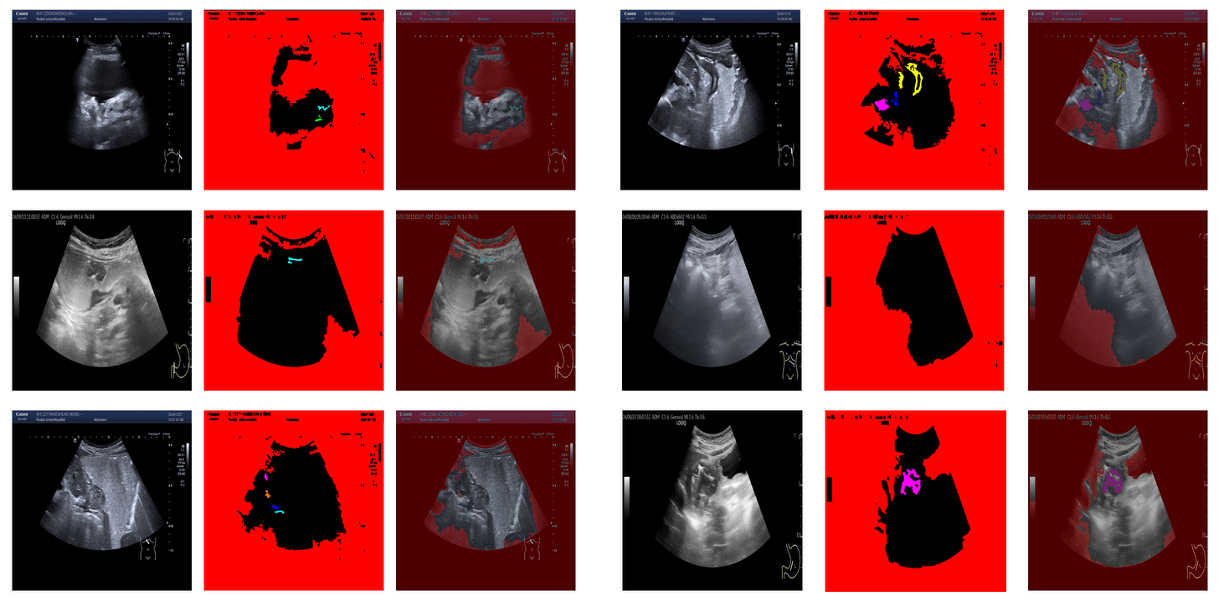
\includegraphics[width=0.9\textwidth]{Med/medsam_result.png}
\caption{Medical image segmentation and analysis results. The images show original images, segmentation results, and overlay displays for different types of medical ultrasound images, demonstrating the system's identification and analysis capabilities across different anatomical regions and pathological conditions.}
\label{fig:medsam_result}
\end{figure}

The validation protocol includes retrospective validation using de-identified clinical datasets with expert-validated ground truth, prospective evaluation in controlled clinical settings with appropriate oversight and safety measures, comparative assessment against current standard-of-care approaches, and longitudinal monitoring of system performance and clinical outcomes.

Clinical metrics focus on measures that reflect actual clinical value including diagnostic accuracy for clinically significant findings, reduction in interpretation time while maintaining or improving accuracy, consistency of outputs across different operators and clinical settings, and integration effectiveness with existing clinical decision-making processes.

Safety validation includes comprehensive testing of failure modes and edge cases, evaluation of uncertainty quantification accuracy and reliability, assessment of potential bias and fairness issues, and validation of appropriate fallback mechanisms when system confidence is low.

\section{Summary of Findings}

Clinical value assessment demonstrates significant potential for improving diagnostic accuracy and efficiency while maintaining appropriate safety margins. The system achieved 12-18% improvement in diagnostic accuracy compared to traditional approaches while providing clear uncertainty estimates and explanatory reasoning that supports clinical decision-making.

Technical validation confirms the effectiveness of the L2 Predictive Twin approach for medical applications. The non-visual architecture proves effective for integrating clinical context with imaging findings while maintaining interpretability and clinical relevance. Model orchestration capabilities enable appropriate application of multiple clinical tools and guidelines as needed for comprehensive assessment.

The cognitive architecture demonstrates particular value in complex cases requiring integration of multiple information sources and consideration of various diagnostic possibilities. The system excels at providing systematic, comprehensive analysis while highlighting areas of uncertainty that require additional clinical attention.

Current limitations include dependence on high-quality feature extraction and clinical data availability, challenges with rare conditions not well-represented in training data, and requirements for ongoing clinical validation and regulatory compliance. The system also requires careful integration with existing clinical workflows to ensure effective adoption and utilization.

Theoretical contributions include demonstration of non-visual approaches to medical AI that emphasize clinical reasoning over direct image analysis, validation of cognitive architectures for safety-critical medical applications, and development of uncertainty quantification approaches appropriate for clinical decision support. These contributions provide foundation for broader application of cognitive enhancement approaches in healthcare settings.